\documentclass{harvardml}

% Authors: 
% Edited by: Mark Goldstein + others (jan 2018)
% Edited by: Amir Shanehsazzadeh, Andrew Kim, Nari Johnson (Jan 2021)
% Edited by: Max Guo, Raphael Pellegrin, Katherine Tian (Jan 2022)
% Edited once more by: William Tong (Jan 2023) + Skyler Wu (Jan 2023)
% Edited once more by: Jeffrey Xu (Jan 2024) + Gabriel Sun (Jan 2024)

% Adapted from CS281 Fall 2019 section 0 notes

% This tex file relies on
% the presence of two files:
% harvardml.cls and common.sty

\course{CS181-s24}
\assignment{Homework \#0}
\duedate{January 26, 2024 at 11:59 PM}

\usepackage{comment}
\usepackage{url}
\usepackage{float}
\usepackage{amsfonts, amsmath, amsthm}
\usepackage{listings}
\usepackage[shortlabels]{enumitem}
\usepackage{hyperref}
\usepackage{etoolbox}
\usepackage{color}
\usepackage{listings}
\usepackage{xcolor}

\lstdefinestyle{mystyle}{
    backgroundcolor=\color{white},   
    commentstyle=\color{green},
    keywordstyle=\color{blue},
    numberstyle=\tiny\color{blue},
    stringstyle=\color{purple},
    basicstyle=\ttfamily\footnotesize,
    breakatwhitespace=false,         
    breaklines=true,                 
    captionpos=b,                    
    keepspaces=true,                 
    numbers=left,                    
    numbersep=5pt,                  
    showspaces=false,                
    showstringspaces=false,
    showtabs=false,                  
    tabsize=2,
    language=Python,
    frame=single
}
\lstset{style=mystyle}

\theoremstyle{definition}
\newtheorem{defn}{Definition}[section]
\theoremstyle{plain}
\usepackage[textsize=tiny]{todonotes}

% Some useful macros.
\newcommand{\given}{\,|\,}
\newcommand{\R}{\mathbb{R}}
\newcommand{\C}{\mathbb{C}}
\newcommand{\E}{\mathbb{E}}
\newcommand{\var}{\text{Var}}
\newcommand{\cov}{\text{Cov}}
\newcommand{\p}{\partial}
\newcommand{\mba}{\mathbf{a}}
\newcommand{\mbb}{\mathbf{b}}
\newcommand{\mbx}{\mathbf{x}}
\newcommand{\mcX}{\mathcal{X}}
\newcommand{\mcY}{\mathcal{Y}}
\newcommand{\boldw}{\mathbf{w}}
\newcommand{\mbxt}{\tilde{\mathbf{x}}}
\newcommand{\Sigmat}{\tilde{\Sigma}}
\newcommand{\mbz}{\mathbf{z}}
\newcommand{\mbw}{\mathbf{w}}
\newcommand{\mcN}{\mathcal{N}}
\newcommand{\mcP}{\mathcal{P}}
\newcommand{\eps}{\epsilon}
\newcommand{\trans}{\intercal}
\newcommand{\Ut}{\tilde{U}}
\DeclareMathOperator*{\argmax}{arg\,max}
\newcommand{\angstrom}{\textup{\AA}}
\renewcommand{\v}[1]{\mathbf{#1}}


\usepackage{xcolor}
\newcount\Comments  % 0 suppresses notes to selves in text
\Comments = 1
\newcommand{\kibitz}[2]{\ifnum\Comments=1{\color{#1}{#2}}\fi}
\newcommand{\dcp}[1]{\kibitz{blue}{[DCP: #1]}}


% Solution environment
\newenvironment{solution}
  {\color{blue}\section*{Solution}}
{}


\begin{document}


\noindent Welcome to CS181! The purpose of this assignment is to help assess your readiness for this course.  It will be graded for completeness and effort.  \textbf{Areas of this assignment that are difficult are an indication of areas in which \emph{you} need to self-study. During the term, the staff will be prioritizing support for new material taught in CS181 over teaching prerequisites.}

\begin{enumerate}
    \item Please type your solutions after the corresponding problems using this \LaTeX\ template, and start each problem on a new page.
    \item Please submit the \textbf{writeup PDF to the Gradescope assignment `HW0'}. Remember to assign pages for each question.
    \item Please submit your \textbf{\LaTeX\ file and code files (i.e., anything ending in \texttt{.py}, \texttt{.ipynb}, or \texttt{.tex}) to the Gradescope assignment `HW0 - Supplemental'}. 
\end{enumerate}

\newpage
\begin{problem}[Modeling Linear Trends - Linear Algebra Review]
In this class we will be exploring the question of ``how do we model the trend in a dataset" under different guises. In this problem, we will explore the algebra of modeling a linear trend in data. We call the process of finding a model that capture the trend in the data, ``fitting the model."\\

\noindent \textbf{Learning Goals:} In this problem, you will practice translating machine learning goals (``modeling trends in data") into mathematical formalism using linear algebra. You will explore how the right mathematical formalization can help us express our modeling ideas unambiguously and provide ways for us to analyze different pathways to meeting our machine learning goals.\\

\noindent Let's consider a dataset consisting of two points $\mathcal{D} = \{(x_1, y_1), (x_2, y_2)\}$, where $x_n, y_n$ are scalars for $n=1, 2$. Recall that the equation of a line in 2-dimensions can be written: $y = w_0 + w_1x$. 
\begin{enumerate}
    \item Write a system of linear equations determining the coefficients $w_0, w_1$ of the line passing through the points in our dataset $\mathcal{D}$ and analytically solve for $w_0, w_1$ by solving this system of linear equations (i.e., using substitution). Please show your work.
    \item Write the above system of linear equations in matrix notation, so that you have a matrix equation of the form $\mathbf{y} = \mathbf{X}\mathbf{w}$, where $\mathbf{y}, \mathbf{w} \in \mathbb{R}^2$ and $\mathbf{X} \in \mathbb{R}^{2\times 2}$. For full credit, it suffices to write out what $\mathbf{X}$, $\mathbf{y}$, and $\mathbf{w}$ should look like in terms of $x_1$, $x_2$, $y_1$, $y_2$, $w_0$, $w_1$, and any other necessary constants. Please show your reasoning and supporting intermediate steps.
    \item Using properties of matrices, characterize exactly when an unique solution for  $\mathbf{w}=\left(w_0 \; w_1 \right)^{T}$ exists. In other words, what must be true about your dataset in order for there to be a unique solution for $\mathbf{w}$? When the solution for $\mathbf{w}$ exists (and is unique), write out, as a matrix expression, its analytical form (i.e., write $\mathbf{w}$ in terms of $\mathbf{X}$ and $\mathbf{y}$).
    
    Hint: What special property must our $\mathbf{X}$ matrix possess? What must be true about our data points in $\mathcal{D}$ for this special property to hold?
    \item Compute $\mathbf{w}$ by hand via your matrix expression in (3) and compare it with your solution in (1). Do your final answers match? What is one advantage for phrasing the problem of fitting the model in terms of matrix notation? 
    \item In real-life, we often work with datasets that consist of hundreds, if not millions, of points. In such cases, does our analytical expression for $\mathbf{w}$ that we derived in (3) apply immediately to the case when $\mathcal{D}$ consists of more than two points? Why or why not?
\end{enumerate}
    
\end{problem}

\newpage


\begin{solution}
\color{black}

\noindent \textbf{1.}
To determine the coefficients \( w_0 \) and \( w_1 \) of the line passing through the two points in the dataset \( \mathcal{D} = \{ (x_1, y_1), (x_2, y_2) \} \), we will use the general equation of a line in 2D: \( y = w_0 + w_1 x \). 
For each point in \( \mathcal{D} \), we substitute \( x \) and \( y \) with their respective values to form a system of linear equations:
\medskip

For \( (x_1, y_1) \), the equation is \( y_1 = w_0 + w_1 x_1 \).
\smallskip

For  \( (x_2, y_2) \), the equation is \( y_2 = w_0 + w_1 x_2 \).

\medskip
So, our system of linear equations is:

\[ y_1 = w_0 + w_1 x_1 \]
\[ y_2 = w_0 + w_1 x_2 \]

Now, let's solve this system for \( w_0 \) and \( w_1 \) using substitution. From the first equation, we can express \( w_0 \) in terms of \( w_1 \):

\[ w_0 = y_1 - w_1 x_1 \]

Substituting the above expression for \( w_0 \) into the second equation:

\[ y_2 = (y_1 - w_1 x_1) + w_1 x_2 \]

Rearranging and solving for \( w_1 \):

\[ y_2 = y_1 + w_1 (x_2 - x_1) \]
\[ w_1 (x_2 - x_1) = y_2 - y_1 \]
\[ w_1 = \frac{y_2 - y_1}{x_2 - x_1} \]

After finding \( w_1 \), we substitute the expression back into the expression for \( w_0 \) to find \( w_0 \):

\[ w_0 = y_1 - w_1 x_1 \]
\[ w_0 = y_1 - \frac{y_2 - y_1}{x_2 - x_1} x_1 .\]

\bigskip
\noindent \textbf{2.}
We have two linear equations derived from the two points \((x_1, y_1)\) and \((x_2, y_2)\):

\[y_1 = w_0 + w_1 x_1\]
\[y_2 = w_0 + w_1 x_2\]

\(\mathbf{y}\) is the vector of outputs. In this case, \(\mathbf{y}\) is:
\[\mathbf{y} = \begin{bmatrix} y_1 \\ y_2 \end{bmatrix}\]

\(\mathbf{w}\) is the vector of unknown coefficients. So, \(\mathbf{w}\) is:
\[\mathbf{w} = \begin{bmatrix} w_0 \\ w_1 \end{bmatrix}\]

\(\mathbf{X}\) is the matrix of inputs. Each row in \(\mathbf{X}\) corresponds to a different equation, and each column corresponds to a coefficient in \(\mathbf{w}\). Therefore, \(\mathbf{X}\) is:
\[\mathbf{X} = \begin{bmatrix} 1 & x_1 \\ 1 & x_2 \end{bmatrix}\]

So, in matrix form, the system of equations becomes:

\[\begin{bmatrix} y_1 \\ y_2 \end{bmatrix} = \begin{bmatrix} 1 & x_1 \\ 1 & x_2 \end{bmatrix} \begin{bmatrix} w_0 \\ w_1 \end{bmatrix}.\]

\bigskip
\noindent \textbf{3.}
A unique solution for \(\mathbf{w} = (w_0, w_1)^T\) in the matrix equation \(\mathbf{y} = \mathbf{Xw}\) exists when the matrix \(\mathbf{X}\) is invertible. 

For the matrix \(\mathbf{X} = \begin{bmatrix} 1 & x_1 \\ 1 & x_2 \end{bmatrix}\), invertibility depends on its determinant being non-zero. The determinant of \(\mathbf{X}\) is calculated as \(\text{det}(\mathbf{X}) = x_2 - x_1\). Therefore, for \(\mathbf{X}\) to be invertible, \(x_1\) and \(x_2\) must be distinct, i.e., \(x_1 \neq x_2\). This condition ensures that the two points in the dataset \(\mathcal{D} = \{(x_1, y_1), (x_2, y_2)\}\) are not vertically aligned.

\medskip
When \(\mathbf{X}\) is invertible, the unique solution \(\mathbf{w}\) can be found using the matrix inverse of \(\mathbf{X}\). The solution is given by \(\mathbf{w} = \mathbf{X}^{-1}\mathbf{y}\).

\bigskip
\noindent \textbf{4.}
To solve for \(\mathbf{w}\), we need the inverse of \(\mathbf{X}\), denoted as \(\mathbf{X}^{-1}\). The inverse of a \(2 \times 2\) matrix \(\mathbf{A} = \begin{bmatrix} a & b \\ c & d \end{bmatrix}\) is given by 
   \[ \mathbf{A}^{-1} = \frac{1}{ad - bc} \begin{bmatrix} d & -b \\ -c & a \end{bmatrix} \]
   For \(\mathbf{X}\), we have \(a = 1\), \(b = x_1\), \(c = 1\), and \(d = x_2\). The determinant \(ad - bc = x_2 - x_1\). Assuming \(x_1 \neq x_2\), the inverse of \(\mathbf{X}\) is:
   \[ \mathbf{X}^{-1} = \frac{1}{x_2 - x_1} \begin{bmatrix} x_2 & -x_1 \\ -1 & 1 \end{bmatrix} \]

For \(\mathbf{X} = \begin{bmatrix} 1 & x_1 \\ 1 & x_2 \end{bmatrix}\) and \(\mathbf{y} = \begin{bmatrix} y_1 \\ y_2 \end{bmatrix}\), the solution \(\mathbf{w}\) is calculated as:

\[
\mathbf{X}^{-1}\mathbf{y} = \mathbf{w} = \begin{bmatrix} w_0 \\ w_1 \end{bmatrix} = \begin{bmatrix} -\frac{x_1 y_2}{-x_1 + x_2} + \frac{x_2 y_1}{-x_1 + x_2} \\ -\frac{y_1}{-x_1 + x_2} + \frac{y_2}{-x_1 + x_2} \end{bmatrix}
\]

Above is valid as long as \(x_1 \neq x_2\), ensuring that the matrix \(\mathbf{X}\) is invertible and a unique solution for \(\mathbf{w}\) exists.

\bigskip
\bigskip
We derived \(w_1\) and \(w_0\) directly from the system of linear equations:
     \[ w_1 = \frac{y_2 - y_1}{x_2 - x_1} \]
     \[ w_0 = y_1 - \left(\frac{y_2 - y_1}{x_2 - x_1}\right) x_1 \]

The solution using matrix inversion was:
     \[ \mathbf{w} = \begin{bmatrix} -\frac{x_1 y_2}{-x_1 + x_2} + \frac{x_2 y_1}{-x_1 + x_2} \\ -\frac{y_1}{-x_1 + x_2} + \frac{y_2}{-x_1 + x_2} \end{bmatrix} \]

This translates to:
\[ w_0 = -\frac{x_1 y_2}{-x_1 + x_2} + \frac{x_2 y_1}{-x_1 + x_2} \]
\[ w_1 = -\frac{y_1}{-x_1 + x_2} + \frac{y_2}{-x_1 + x_2} \]

For \(w_1\):

Part 1: \[w_1 = \frac{y_2 - y_1}{x_2 - x_1}\]

Part 3: \[w_1 = -\frac{y_1}{-x_1 + x_2} + \frac{y_2}{-x_1 + x_2} = \frac{y_2 - y_1}{x_2 - x_1}\]


For \(w_0\):

Part 1: \[w_0 = y_1 - \left(\frac{y_2 - y_1}{x_2 - x_1}\right) x_1\]

Part 3: \[w_0 = -\frac{x_1 y_2}{-x_1 + x_2} + \frac{x_2 y_1}{-x_1 + x_2}\] 
Simplifying:
    \[ w_0 = \frac{-x_1 y_2 + x_2 y_1}{x_2 - x_1} \]
    \[ w_0 = \frac{x_2 y_1 - x_1 y_2}{x_2 - x_1} \]
    \[ w_0 = y_1 - \frac{x_1(y_2 - y_1)}{x_2 - x_1} \]
    \[ w_0 = y_1 - \left(\frac{y_2 - y_1}{x_2 - x_1}\right) x_1 \]
\medskip


It is evident that the expression for \(w_0\) from the matrix method is the same as that from the direct calculation method.
We can conclude that both part 1 and 3 are correct and consistent. 

Matrix notation in linear regression offers an interesting way to understand the problem not only algebraically but also geometrically. It connects the problem to linear algebra concepts, such as linear transformations, vector spaces, orthogonality, etc., which can provide deeper insights to help us analyze our data-points.

\bigskip
\noindent \textbf{5.}
The analytical expression for \(\mathbf{w}\) we derived in part 3, which assumes exactly two points, does not directly apply for multiple points. With more than two points, the system of equations becomes overdetermined. For a system of equations problem with \(n\) points, where \(n > 2\), in a two-dimensional space, you have \(n\) equations but only 2 unknowns, namely the coefficients \(w_0\) and \(w_1\)). This system cannot be solved using the straightforward matrix inversion approach we used for two points, because the matrix \(\mathbf{X}\) in this case will be \(n \times 2\), which is not square and thus not invertible.
\end{solution}

\color{black}
\newpage


\begin{problem}[Optimizing Objectives - Calculus Review]
In this class, we will write real-life goals we want our model to achieve into a mathematical expression and then find the optimal settings of the model that achieves these goals. The formal framework we will employ is that of mathematical optimization. Although the mathematics of optimization can be quite complex and deep, we have all encountered basic optimization problems in our first calculus class!\\

\noindent \textbf{Learning Goals:} In this problem, we will explore how to formalize real-life goals as mathematical optimization problems. We will also investigate under what conditions these optimization problems have solutions.\\

\noindent In her most recent work-from-home shopping spree, Nari decided to buy several house plants. \textit{Her goal is to make them to grow as tall as possible.} After perusing the internet, Nari learns that the height $y$ in mm of her Weeping Fig plant can be directly modeled as a function of the oz of water $x$ she gives it each week:
$$y = - 3x^2 + 72x + 70.$$
\begin{enumerate}
    \item Based on the above formula, is Nari's goal achievable: does the plant have a maximum height? Why or why not? Does her goal have a unique solution - i.e. is there one special watering schedule that would acheive the maximum height (if it exists)?
    
    Hint: plot this function. In your solution, words like ``convex" and ``concave" may be helpful.
    \item Using calculus, find how many oz per week should Nari water her plant in order to maximize its height. With this much water, how tall will her plant grow?

    Hint: solve analytically for the critical points of the height function (i.e., where the derivative of the function is zero).  For each critical point, use the second-derivative test to identify if each point is a  max or min point, and use arguments about the global structure (e.g., concavity or convexity) of the function to argue whether this is a local or global optimum.
\end{enumerate}
Now suppose that Nari want to optimize both the amount of water $x_1$ (in oz) \textit{and} the amount of direct sunlight $x_2$ (in hours) to provide for her plants. After extensive research, she decided that the height $y$ (in mm) of her plants can be modeled as a two variable function:

$$y = f(x_1, x_2) = \exp\left(-(x_1 - 2)^2 - (x_2 - 1)^2 \right)$$
\begin{enumerate}
    \setcounter{enumi}{2}
    \item Using \texttt{matplotlib}, visualize in 3D the height function as a function of $x_1$ and $x_2$ using the \texttt{plot\_surface} utility for $(x_1, x_2) \in (0, 6) \times (0, 6)$. Use this visualization to argue why there exists a unique solution to Nari's optimization problem on the specified intervals for $x_1$ and $x_2$.

    Remark: in this class, we will learn about under what conditions do \textit{multivariate} optimization problems have unique global optima (and no, the second derivative test doesn't exactly generalize directly). Looking at the visualization you produced and the expression for $f(x_1, x_2)$, do you have any ideas for why this problem is guaranteed to have a global maxima? You do not need to write anything responding to this -- this is simply food for thought and a preview for the semester.
\end{enumerate}
\end{problem}

\newpage


\begin{solution}
\color{black}
\noindent \textbf{1.}

\begin{figure}[h]
    \centering
    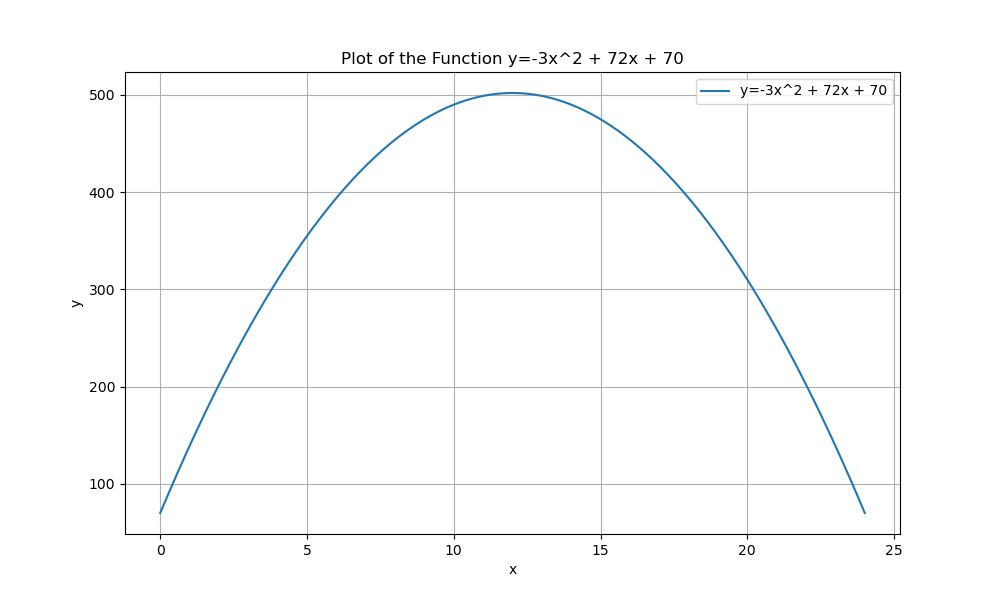
\includegraphics[width=0.75\linewidth]{parabola.png}
    \caption{resulting parabola}
    \label{fig:enter-label}
\end{figure}
When we look at the equation $y=-3 x^2+72 x+70$, it is evident that it's a quadratic function with a negative leading coefficient, -3. This means the graph of the function is a downward-opening parabola, which has a maximum point, vertex. 

\medskip
The maximum height of the plant is found at the vertex of the parabola. The x-coordinate of the vertex of a parabola given by \( y = ax^2 + bx + c \) is found using the formula \( x = -\frac{b}{2a} \). Since \( a = -3 \) and \( b = 72 \), the x-coordinate of the vertex is:
\[ x = -\frac{72}{2 \times -3} = -\frac{72}{-6} = 12 \]

As we see above, the unique watering schedule to achieve the maximum height is to give the plant 12 oz of water each week.

\bigskip
\noindent \textbf{2.}
We need to find the critical points of the height function \( y = -3x^2 + 72x + 70 \) and then determine which of these points corresponds to a maximum.

\medskip
The derivative of the height function with respect to x represents the rate of change of the plant's height with respect to the amount of water.
\medskip
The derivative \( y' \) of \( y = -3x^2 + 72x + 70 \) is:
     \[ y' = -6x + 72 \]
To find critical points, we set the derivative equal to zero and solve for \( x \):
     \[ -6x + 72 = 0 \]
     \[ -6x = -72 \]
     \[ x = 12 \]

Then we use the second-derivative test to determine whether this critical point is a maximum or minimum. The second derivative \( y'' \) of \( y = -3x^2 + 72x + 70 \) is:
     \[ y'' = -6 \]
Since \( y'' \) is negative, the function is concave down at this point, which means that the critical point \( x = 12 \) is a maximum.

\medskip
Since the vertex is a downward-opening parabola, any local maximum is also a global maximum.
We can conclude that the critical point \( x = 12 \) not only represents a local maximum but also the global maximum height of the plant.

\medskip
To find the maximum height of the plant, substitute \( x = 12 \) into the original equation:
     \[ y = -3(12)^2 + 72(12) + 70 \]

When Neri waters her Weeping Fig plant with 12 oz of water per week, the plant will reach its maximum height of 502 mm.

\bigskip
\noindent \textbf{3.}

\begin{figure}[h]
    \centering
    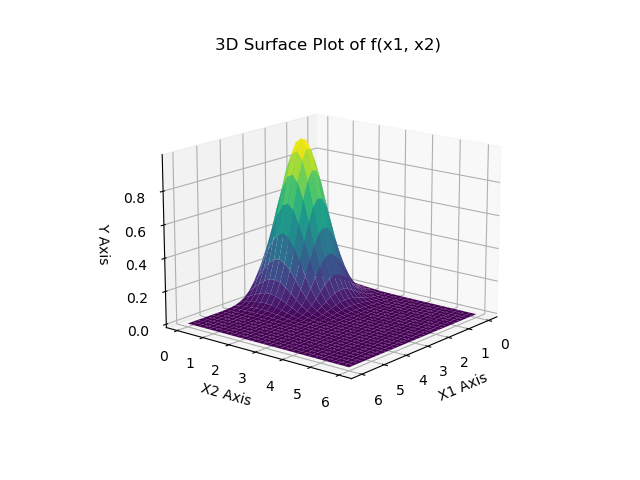
\includegraphics[width=0.75\linewidth]{Figure_2.png}
    \caption{Resulting Surface plot}
    \label{fig:enter-label}
\end{figure}

The function is based on the exponential of negative squares, which typically forms a bell-shaped curve, as seen on the graph. This kind of curve generally has a single peak, especially when the squares are centered around specific values (in this case, \(x_1 = 2\) and \(x_2 = 1\)).

\medskip
The maximum point of this function is where the exponent \( -\left(x_1 - 2\right)^2 - \left(x_2 - 1\right)^2 \) is maximized, which happens at the point \(x_1 = 2\) and \(x_2 = 1\). This point represents the peak. Given the nature of the function, this peak or maximum point is unique. The function decreases exponentially as we move away from the peak in any direction. Therefore, within the specified intervals of \(x_1\) and \(x_2\), the graph will not have any other local maxima.

\medskip
The graph above shows a single, prominent peak with the height decreasing as we move away from this peak in any direction within the specified intervals. This visual confirmation supports our mathematical understanding that there is one, and only one, maximum height that the plant can achieve given the right combination of water (\(x_1\)) and sunlight (\(x_2\)).
\end{solution}


\color{black}

\begin{problem}[Reasoning about Randomness - Probability and Statistics Review]
In this class, one of our main focuses is to model the unexpected variations in real-life phenomena using the formalism of random variables. In this problem, we will use random variables to model how much time it takes an USPS package processing system to process packages that arrive in a day.\\

\noindent \textbf{Learning Goals:} In this problem, you will analyze random variables and their distributions both analytically and computationally. You will also practice drawing connections between said analytical and computational conclusions.\\

\noindent Consider the following model for packages arriving at the US Postal Service (USPS):
\begin{itemize}
    \item Packages arrive randomly in any given hour according to a Poisson distribution. That is, the number of packages in a given hour $N$ is distributed $Pois(\lambda)$, with $\lambda = 3$.
    \item Each package has a random size $S$ (measured in $in^3$) and weight $W$ (measured in pounds), with joint distribution
    $$(S, W)^{T} \sim \mathcal{N}\left( \boldsymbol{\mu}, \boldsymbol{\Sigma}\right) \text{, with } \boldsymbol{\mu} = \begin{bmatrix} 120 \\ 4 \end{bmatrix} \text{ and } \boldsymbol{\Sigma} = \begin{bmatrix} 1.5 & 1 \\ 1 & 1.5 \end{bmatrix}.$$
    \item Processing time $T$ (in seconds) for each package is given by $T = 60 + 0.6 W + 0.2 S + \epsilon$, where $\epsilon$ is a random noise variable with Gaussian distribution $\epsilon \sim \mathcal{N}(0, 5)$.
\end{itemize}
For this problem, you may find the \texttt{multivariate\_normal} module from \texttt{scipy.stats} especially helpful. You may also find the \texttt{seaborn.histplot} function quite helpful. 
\begin{enumerate}
    \item Perform the following tasks:
    \begin{enumerate}
        \item Visualize the Bivariate Gaussian distribution for the size $S$ and weight $W$ of the packages by sampling 500 times from the joint distribution of $S$ and $W$ and generating a bivariate histogram of your $S$ and $W$ samples.
        \item Empirically estimate the most likely combination of size and weight of a package by finding the bin of your bivariate histogram (i.e., specify both a value of $S$ and a value of $W$) with the highest frequency. A visual inspection is sufficient -- you do not need to be incredibly precise.  How close are these empirical values to the theoretical expected size and expected weight of a package, according to the given Bivariate Gaussian distribution?
    \end{enumerate}
    \item For 1001 evenly-spaced values of $W$ between $0$ and $10$, plot $W$ versus the joint Bivariate Gaussian PDF $p(W, S)$ with $S$ fixed at $S=118$. Repeat this procedure for $S$ fixed at $S=122$. Comparing these two PDF plots, what can you say about the correlation of random variables $S$ and $W$?
    \item Give one reason for why the Gaussian distribution is an appropriate model for the size and weight of packages. Give one reason for why it may not be appropriate.
    \item Because $T$ is a linear combination of random variables, it itself is a random variable. Using properties of expectations and variance, please compute $\mathbb{E}(T)$ and $\mathrm{Var}(T)$ analytically.
    \item Let us treat the \textit{total} amount of time it takes to process \textit{all} packages received at the USPS office within \textit{an entire day} (assuming a single day is $24$ hours long) as a random variable $T^{*}$. 
    \begin{enumerate}
        \item Write a function to simulate draws from the distribution of $T^{*}$. 
        \item Using your function, empirically estimate the mean and standard deviation of $T^{*}$ by generating $1000$ samples from the distribution of $T^{*}$.
    \end{enumerate}
\end{enumerate}
\end{problem}

\newpage

\begin{solution}
\color{black}
\noindent \textbf{1.}

\bigskip
\noindent \textbf{(a)}

\begin{figure}[h]
    \centering
    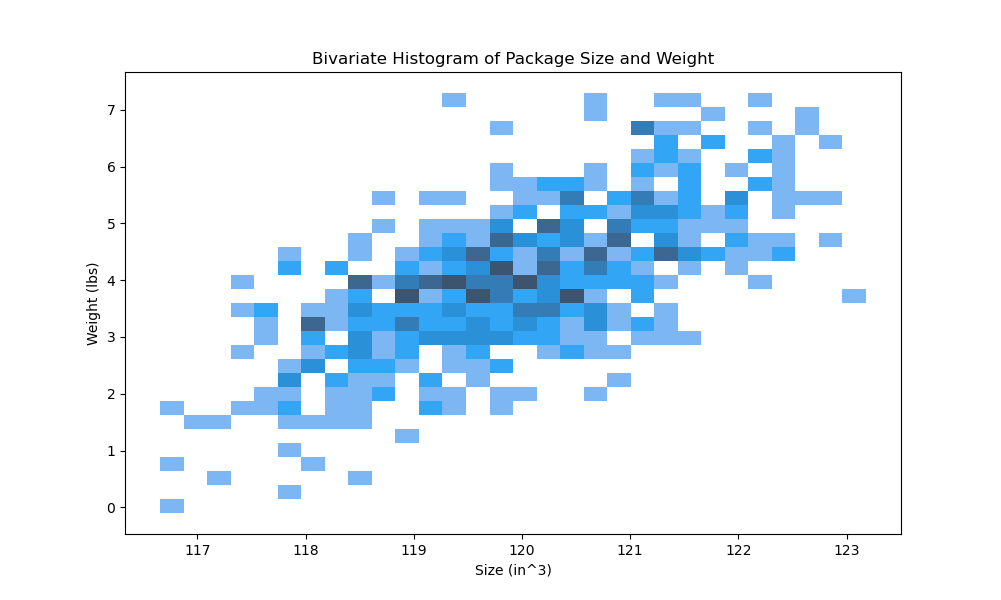
\includegraphics[width=1\linewidth]{histogram.png}
    \caption{resulting plot}
    \label{fig:enter-label}
\end{figure}

\noindent \textbf{(b)}
From the graph (Fig. 3),
Size \(S\) between approximately 119 and 121 cubic inches.
Weight \(W\) between approximately 3.5 and 4.5 pounds.

\medskip
The exact center of the darkest bin would be the midpoint of these ranges, which we could estimate as \(S \approx 120\) cubic inches and \(W \approx 4\) pounds, very close to the theoretical expected values. This close match between the empirical and theoretical values is consistent with the properties of the Gaussian distribution, where sample means tend to converge to the theoretical means as sample size increases (in this case, 500 samples).

\bigskip
\noindent \textbf{2.}

\begin{figure}[h]
    \centering
    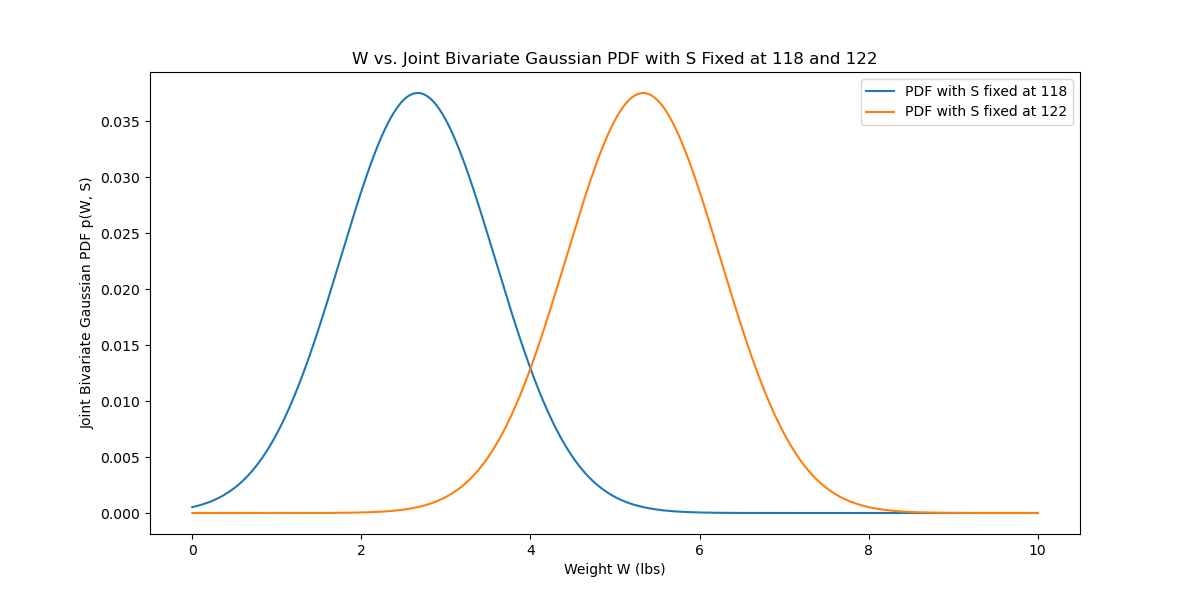
\includegraphics[width=0.75\linewidth]{mow.png}
    \caption{Resulting graph}
    \label{fig:enter-label}
\end{figure}
When \( S \) is fixed at 118, the peak of the PDF curve for \( W \) is shifted slightly to the left compared to when \( S \) is fixed at 122 (Fig. 4).

\medskip
The fact that the peaks are at different weights for different fixed sizes indicates that the size and weight are correlated. If size and weight were independent, the PDF curves would have the same shape and the same peak position regardless of the fixed size.

\medskip
The positive correlation is further evidenced by the fact that the peak corresponding to \( S = 122 \) is higher for \( W \), suggesting that larger sizes are associated with greater weights. Comparing the two PDF plots, we can see that the variables \( S \) and \( W \) are indeed correlated, and as \( S \) increases, the most probable weight \( W \) also increases. The PDF plots reflect the positive covariance between \( S \) and \( W \) given in the covariance matrix \(\boldsymbol{\Sigma}\).


\bigskip
\noindent \textbf{3.}
The Gaussian distribution is often an appropriate model for physical measurements like size and weight due to the Central Limit Theorem. In practice, the size and weight of packages are effected by numerous small, independent factors, such as contents, packaging material, air pockets, etc., and the total effect of these factors can lead to a normal distribution for the overall size and weight.

\medskip
The Gaussian distribution is unbounded. However, both the size and weight of packages are strictly non-negative. If the mean of the distribution is close to zero or the variance is large, the Gaussian model might predict a non-trivial probability for physically impossible negative values. In cases like that, a different distribution that is bounded at zero, for example a log-normal or Gamma distribution, might be more appropriate.

\bigskip
\noindent \textbf{4.}
The processing time \(T\) is given by:

\[ T = 60 + 0.6W + 0.2S + \epsilon \]

where \(\epsilon\) is a random noise variable with Gaussian distribution \(\epsilon \sim \mathcal{N}(0,5)\), and \(S\) and \(W\) have a joint Gaussian distribution with means 120 and 4, and covariance matrix \(\Sigma\).

\medskip
The expectation \(\mathbb{E}(T)\) is linear, so we can compute it as:
\[ \mathbb{E}(T) = 60 + 0.6\mathbb{E}(W) + 0.2\mathbb{E}(S) + \mathbb{E}(\epsilon) \]

Since \(\epsilon\) has a mean of 0, \(\mathbb{E}(W) = 4\), and \(\mathbb{E}(S) = 120\), we get:

\[ \mathbb{E}(T) = 60 + 0.6 \cdot 4 + 0.2 \cdot 120 + 0 \]
\[ \mathbb{E}(T) = 60 + 2.4 + 24 \]
\[ \mathbb{E}(T) = 86.4 \]

The variance \(\operatorname{Var}(T)\) can be computed using the fact that the variance of a constant is 0 and the variance of a sum of independent variables is the sum of their variances.

\[ \operatorname{Var}(T) = \operatorname{Var}(60) + \operatorname{Var}(0.6W) + \operatorname{Var}(0.2S) + \operatorname{Var}(\epsilon) \]
\[ \operatorname{Var}(T) = 0 + 0.6^2 \operatorname{Var}(W) + 0.2^2 \operatorname{Var}(S) + \operatorname{Var}(\epsilon) \]

Given the variances from the covariance matrix \(\Sigma\), where \(\operatorname{Var}(S) = 1.5\) and \(\operatorname{Var}(W) = 1.5\), and \(\operatorname{Var}(\epsilon) = 5\), we get:
\[ \operatorname{Var}(T) = 0.6^2 \cdot 1.5 + 0.2^2 \cdot 1.5 + 5 \]
\[ \operatorname{Var}(T) = 0.36 \cdot 1.5 + 0.04 \cdot 1.5 + 5 \]
\[ \operatorname{Var}(T) = 0.54 + 0.06 + 5 \]
\[ \operatorname{Var}(T) = 5.6 \]

The expected processing time \(\mathbb{E}(T)\) is 86.4 seconds and the variance of the processing time \(\operatorname{Var}(T)\) is 5.6 seconds^2.

\medskip
\noindent \textbf{5.}

\medskip
\noindent \textbf{(b)}

Empirical Mean of T*: 6243.791337889397

Empirical Standard Deviation of T*: 749.9724374504037

\end{solution} 


\end{document}